\chapter{ Description of the model \label{ch:numero_uno}}
\section{An invitation to algebraic representation of cell boundaries}
The use of signed distance fields (SDFs) to model organic sufaces
is a time honoured graphical technique used, for example, by Pixar
Animation Studios to model hair in \textit{The Incredibles} 
(see \cite{petrovic2005volumetric}). The idea is to define a 
function which represents the closest distance from the query point
to a point on the surface of the object that is to be represented. 
If the query point is outside, the SDF is positive,
the SDF is zero on the surface and negative inside. SDFs can be 
rendered within traditional graphics pipelines (such as OpenGL or Vulkan)
using raymarching, a method that takes place within shader programs and 
is therefore meshless. The formulae defining SDFs for common 2D and 3D 
shapes are easy to find online, see \cite{key}. In this thesis,
we do not use signed distance fields based on the practical 
reason that their definitions usually involve square roots
which are slow to compute. We employ very similar formula
without the square roots, which yield the same level sets (in 2D)
but are fast to compute.
\\

To motivate the primary mechanism by which cells will undergo mitosis 
in this thesis, we consider a toy example in which the level sectios of the equations for
a pair of ellipses undergo a catastrophic topological change as one real parameter 
changes, namely the distance $d$ between their centers. We start by considering 
the equations for two spheres which 
begin as coincident and move apart as the parameter $d$ becomes larger. 
The equations that represent the individual cells are
\begin{equation*}
    f_1(x,y,z) = \left( \frac{x+d}{p} \right)^2 + \left( \frac{y}{q} \right)^2 - 1,
\end{equation*}
\begin{equation*}
    f_2(x,y,z) = \left( \frac{x-d}{p} \right)^2 + \left( \frac{y}{q} \right)^2 - 1,
\end{equation*}
where $p=1.0 L_0$ and $q=0.9 L_0$ are the semi-major radius and semi-minor radius
of the ellispes, respectively, 
and $d$ is the distance bewteen their centers. The aspect ratio is $q/p = 0.9$ and $L_0 = 3.5 \ \mu m$
is the average length of a  saccharomyces cerevisiae (Baker's yeast) cell in ideal conditions (reference).
\\

In order to generate 
the combined algebraic curve for the pair, which, by an abuse of notation, will 
be called the colony SDF from now on, we build the following.
This is done using a what is called a ``union" in computer graphics
(see \cite{fusekvisualization}). This is simply the pointwise minimum,
\begin{equation*}
    f_{\textrm{union}}(x,y,z) = \min(f_1(x,y,z), f_2(x,y,z)).
\end{equation*} 
To get a smooth transition between the cells as they come apart we could alternatively use 
the $\textrm{smoothmin}$ which is defined by a smoothness parameter $s$, as in
\begin{equation*}
    \textrm{smoothmin}(f_1(x,y,z), f_2(x,y,z); s) = -s \log(e^{-f_1(x,y,z)/s} + e^{-f_2(x,y,z)/s}).
\end{equation*}
\begin{figure}[!htb]
    \centering
    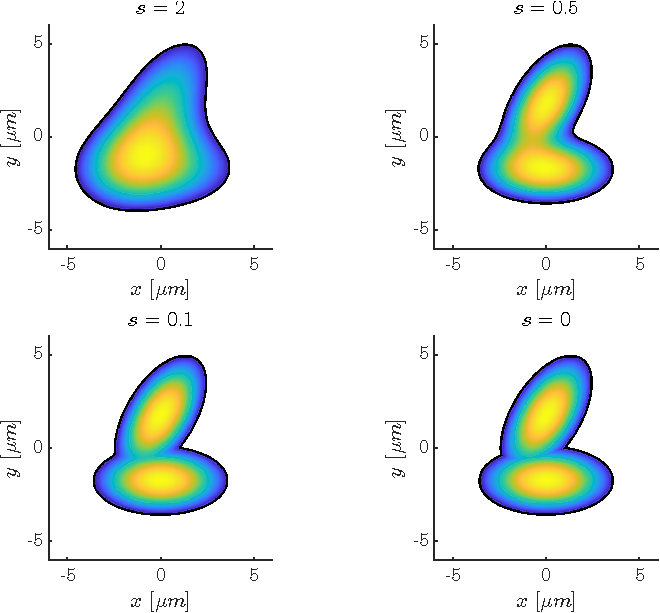
\includegraphics[width=0.8\textwidth]{chapter1/figures/compareSmoothness.pdf}
    \caption{Two ellipses blended with various values of smoothness $s$. The bottom right 
             figure is computed using standard minimum instead of smoothmin. Indeed,
             as $s \rightarrow 0$, the plot looks less smoothed across.}
    \label{fig:compareSmoothness}
\end{figure}
Figure \ref{fig:compareSmoothness} shows the effect of using different values of smoothness
$s$. Ultimately, using smoothmin was abandoned in favour or the computationally quicker \codeword{min},
which does not require the costly evaluation of the natural log and exponential functions.
\\

As shown in figure \ref{fig:mitosisplot}, we have a smooth splitting of a 
cell as the parameter $d$ ranges from $0.0$ to $9.1 \ \mu m$. Here $s$ is the 
smoothing parameter. In order to ensure that only the interior
of the SDF level section was plotted, I set positive entries to \codeword{nan},
which is MATLAB code for \textit{not a number}. The surface plots in figure \ref{fig:mitosisplot}
were produced via the use of MATLAB's \codeword{surf} function which ignores \codeword{nan} entries
in the underlying $Z$ matrix. One additional transformation made before plotting, was to multiply by 
$-1$ to reflect the SDF about the level plane, achieving a positive value inside the biomass.
\begin{figure}[!htb]
    \centering
    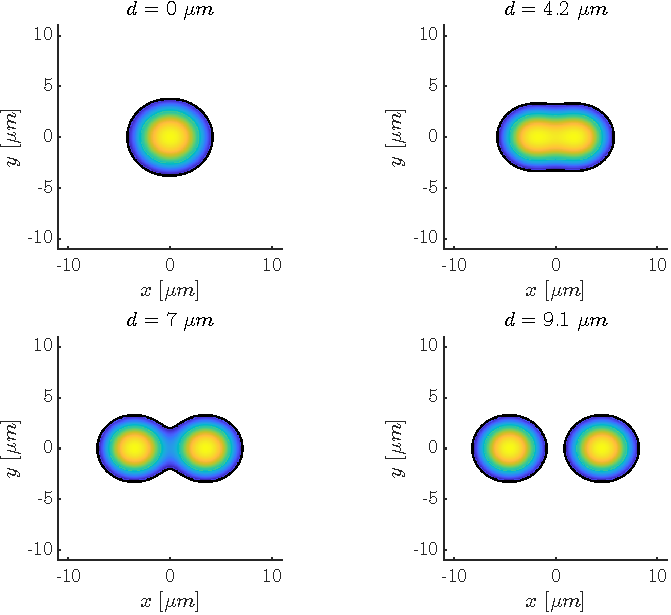
\includegraphics[width=0.8\textwidth]{chapter1/figures/mitosisPlot.pdf}
    \caption{The separation $d$ between two ellipse shapes with $s = 0.5$ and 
    an aspect ratio of $0.9$}
    \label{fig:mitosisplot}
\end{figure}
\\

A signed distance field for an ellipse is used to model Baker's yeast cells which
are in a pseudo-hyphal growth regime.
An ellipse centered at the origin with semi-major dimension $p$ (the $x$ intercept) and
semi-minor dimension $q$ (the $y$ intercept) has an SDF given by
\begin{equation*}
    f(x,y) = \sqrt{ \left( \frac{x}{p} \right)^2 + \left( \frac{y}{q} \right)^2 } - 1.
\end{equation*}
Recall that for computational efficiency we choose to use,
\begin{equation*}
    f(x,y) = \left( \frac{x}{p} \right)^2 + \left( \frac{y}{q} \right)^2  - 1.
\end{equation*}
This is not really a \textit{distance} field because it is 
dimensionless but it will still be called an SDF since it produces the 
elliptical shape all the same. We can also translate and rotate the ellipse, using
\begin{equation*} 
    \Delta \vb{x}' = 
    \begin{bmatrix}
        \cos{\theta} & \sin{\theta} \\
        -\sin{\theta} & \cos{\theta} 
    \end{bmatrix}
    \Delta \vb{x},
\end{equation*}
where $\Delta \vb{x} = (x-x_c) \hat{\vb{i}} + (y-y_c)\hat{\vb{j}} $ and $(x_c,y_c)$ is the
center of the ellipse. We call the components of $\Delta \vb{x} = \Delta x \hat{\vb{i}} +
\Delta y \hat{\vb{j}} $. The above trasnformation is a passive rotation because 
it rotates the whole SDF. The following equation
\begin{equation*}
    f(x,y) = \left[\frac{ (x-x_c)\cos{\theta} + (y-y_c) \sin{\theta}}{p} \right]^2 
        + \left[ \frac{-(x-x_c)\sin{\theta} +(y-y_c) \cos{\theta}}{q} \right]^2 - 1.
\end{equation*}
is used in the custom MATLAB function \codeword{ellipse.m} devloped here. Each individual 
cell has a unique value of $(x_c,y_c,p,q,\theta)$ which we index by $k$. Bringing them all 
together in one function using \codeword{min}, we have the colony SDF given by,
\begin{equation*}
    g(x,y) = \min_{k \in \{1, ..., N_{\textrm{cells}}\}} f_k(x,y),
\end{equation*}
where the individual SDF for each cell is given by 
\begin{equation*}
    f_k(x,y) = \left[\frac{ (x-x_{c,k})\cos{\theta_k} + (y-y_{c,k}) \sin{\theta_k}}{p_k} \right]^2 
        + \left[ \frac{-(x-x_{c,k})\sin{\theta_k} +(y-y_{c,k}) \cos{\theta_k}}{q_k} \right]^2 - 1.
\end{equation*}
Cell colonies can also be built up by combining the SDFs of the individual cells 
using a cumulative $\textrm{smoothmin}$.
\\

Some significant optimsations were made to make sure that the evalution of 
the colony SDF (evaluated via calling \codeword{ellipse}) was as fast as 
possible within the capabilities of MATLAB. These 
optimisations, which were crucial because \codeword{ellipse} is called per time step, 
are commented on in Chapter 2.

\section{Cell colony dynamics with an underlying discrete network}
Now that we have introduced a robust mechanism to represent cell colony 
shape, the question naturally arises about how to represent the time dependence of this 
morphology. To represent the branching dynamics of pseudo-hyphal yeast growth, 
an underlying discrete network which could change node count has been developed.
In order to address the concern of simplicity of 









\section{Mitosis: new cells from old}
In summary, the mechanism of mitosis is a slight of hand, in the sense that
each of the nodes (two nodes per cell) are already there at the simulation
outset. The appearance of growth of the colony coincides with the nodes' progressive
dislodgement from their equality constraints with one another. Of course,
there is no reason why the model could not be modified to add nodes
that were not there to begin with, though such a model would yield
equivalent results.
\\
To interpret the model mathematically, we recall that it was desireable to have
a time parameter $t$ over which the state of the colony could vary. The main 
goal of the thesis was to demonstrate that a system, in this case a yeast colony,
which appears to acquire more dynamical variables (new coordinates for new cells for example)
could be represented by a model with a fixed number of variables which are
initially coincident.
\\
Philosophically, however, the model has some limitations. In reality, we know the growth
of fungal species such as Baker's yeast, is strongly dependent on factors such as temperature
and the environmental conditions that the colony is subjected to. This means 
that the dynamics of cell growth (the collision and interaction as well as the morphology) in 
any large colony system cannot be intrinsically defined. To put it succinctly, the dynamics of 
the colony is strongly coupled to the local environmental conditions.
\\
Does this mean that we can only model biological systems completely if all the conditions 
are incorporated? As per the discussion in the introduction about mathematical modelling,
we aim to consider the simplest viable model. This, in the case of the current work, 
is a model that has two components: a cell colony as discussed in the preceeding section, and 
a nutrient field. Indeed, their coupling determines the dynamics. 
\\
In the discussion, I will suggest ways to relax these limiting assumptions that
are outside the scope of the current work but are nonetheless interesting to consider.
\\
This model, in which the colony appears as the ``unfolding" of a network of nodes
follows on somewhat naturally from the theory of $L$-systems, in which the underlying 
discrete structure of a system is allowed to evolve deterministically based on rules
analogous to cellular automata. A criticism which has been leveled 
(find relevant paper that I read a while ago) at $L$-systems and other deterministic models
of plants for example, is what I call their intrinsic nature. That is, they effectively
rely on the assumption that a biological system's rules for developement are somehow contained
within it's structure (for instance, DNA). It is more fashionable nowadays, and indeed more 
scientifically accurate, to think of a biological system as part of a complex network 
of other organisms and environmental conditions which determine its morphology.
\\
Consider a minimalistic example of modelling the motion of a spherical ball rolling around on a table.
Two spatial paramters $x$ and $y$, together as a tuple are enough to say where it is. However, 
if the ball unexpectately falls from the table, then you would suddenly require
another parameter to describe the state of the system. The value of this classical example
is to demonstrate for $N$ particles and $M$ constraints that may suddenly change, 
we can derive rich and unexpected dynamics.
\\
The best we can hope for is that our parametrisation is somehow dense in the space
of all possible cell colony configurations that we see experimentally. There are even
some exotic cases of cellular sytems in which a single cell can have nontrivial topologies (ask Ed 
about the slime cells which optimise their topology based on nutrient). Therefore, future work 
should focus on representations of dynamic cell geometries that are as free of assumptions as
is conceivable. Once an abstract enough representation of a biological system and its environment
becomes available in the theory, one can use it to study and predict novel morphologies that appear 
in nature. Hopefully it is clear that the present work is just a suggestion of the numerous possibilities
in the area of biolgical morphology viewed in the framework of ``growing geometry''.


\section{Adding in a nutrient field}
The nutrient field is some form of glucose mixture (agar) that is assumed to be given by a reaction-diffusion 
partial differential equation. That is, the nutrient concentration $u(x,y,t)$ is given by
\begin{equation}
    \pdv{u(x,y,t)}{t} = D \left( \frac{\partial^2 u(x,y,t)}{\partial x^2} + 
                          \frac{\partial^2 u(x,y,t)}{\partial y^2} \right) - r u(x,y,t) f(x,y,t)
\end{equation}
where $f(x,y,t)$ is the microscopic biomass density of the cell colony, $D$ is a diffusion
coefficient and $r$ is a constant measuring the rate at which the cells consume nutrient.
The PDE is subjected to a Dirichlet condition, i.e
that the nutrient density vanishes at the boundary. In order to simulate the nutrient field
numerically we use a finite difference on the square grid covering the domain. This is implemented 
using a $5$-point stencil for space and a forward Euler method for time.
\begin{equation}
    \frac{u_{i,j}^{n+1} - u_{i,j}^n}{\Delta t} = 
    D \left( \frac{u_{i+1,j}^{n} - 2 u_{i,j}^n +u_{i-1,j}^n}{h^2} +
             \frac{u_{i,j+1}^{n} - 2 u_{i,j}^n +u_{i,j-1}^n}{h^2} \right)-
             r u_{i,j}^n f_{i,j}^n,
\end{equation}
where $i,j$ take on values in the interior grid points, $n$ is a positive integer time index, 
$h$ is the spatial step (same in $x$ and $y$ directions) and $\Delta t$ is the time increment. See the
figure below for an initial condition set to a sine wave product which vanishes on the boundaries.




\section{Calculating the compactness metric}
A fully grown colony will in general not be perfectly circular in shape.
 In order to measure the roundness of the colony we use the compactness metric used for 
 roundness in image processing (quote Kai use of this metric)
\begin{equation}
  C = \frac{P^2}{4 \pi A},
\end{equation}
where $C \in [1, \infty)$ is $1$ for a circle and can get to large numbers for 
highly branching shapes, $A$ is the colony area, and $P$ is the colony perimeter. 
Both of these are calculated from the formula for the microscopic cell
density which is always given by when $f(x,y,t)$ changes sign. A black and white image 
is produced at each time step using Matlab's function \codeword{bwboundaries} as per
Kai's suggestion. The area then is given by summing up the grid squares that are
inside the implicit shape givcen by $f$ and multiplying by $h^2$. The perimeter
is got by using \codeword{bwboundaries}, which outputs an array of points on the boundary
from which the Euclidean distance between neighbouring points is found and then summed over.

\begin{figure}[h]
    \centering
    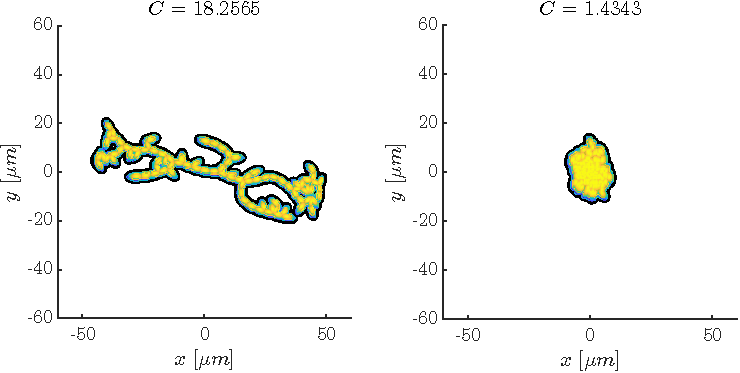
\includegraphics[width=\textwidth]{chapter1/figures/compareCompactness.pdf}
    \caption{A comparsion of high and low compactness}
    \label{fig:compatness_comparison}
\end{figure}
